\documentclass{beamer}

\usepackage[ngerman]{babel}
\usepackage[utf8x]{inputenc}
\usepackage{amsmath,amsfonts,amssymb}
\usepackage{algorithm}
\usepackage[noend]{algpseudocode}

\usepackage{subcaption}

\usepackage[absolute,overlay]{textpos}



\usepackage{kbordermatrix}

\newcommand{\todo}[1]{\textcolor{red}{TODO: #1}}

\setbeamertemplate{bibliography item}[text]
\bibliographystyle{unsrt}


\usetheme{Luebeck}
\usecolortheme{orchid}

\title{Seminar combinatorial optimization}
\subtitle{Approximative algorithms for the multiway cut problem}
\author{Jan Lammel}

\begin{document}
	
\frame{\titlepage}

\frame{
	\frametitle{Table of contents}
	\tableofcontents[hideallsubsections]
	
}

\section{Introduction}
\frame{
\frametitle{Introduction}

\begin{textblock}{12}(1,5)
	Until now: \\
	\begin{itemize}
	\item 2 label segmentation (foreground / background)
	\item Efficient via max-flow / min-cut
	\end{itemize}
	
	Now: \\
	\begin{itemize}
	\item Segmentation with arbitrary number of labels
	\item Actual problem is NP-complete
	\item Reduction to small 2-label problems with approximative methods
	\end{itemize}
\end{textblock}
}

\frame{
\frametitle{Introduction}
\todo{Bild + fertige Segmentierung als Motivation was am Ende rauskommen soll.}



}

\section{Mathematical problem formulation}
\subsection{Basic definitions}
\frame{
\frametitle{Basic definitions}

\begin{textblock}{14}(1, 4.5)

	\begin{itemize}
		\item Image consists of pixels $P = \{ 1, 2, ..., m \}$
		\item Segmentation labels $\mathcal{L} = \{l_1,l_ 2, ..., l_k\}$
		\item Each pixel has two statistical values
		\begin{itemize}
			\item hypothesis $f \in \mathcal{L}^m$: \ segmentation label
			\item observation $O$: \qquad \ information in the image (intensities, ...)
		\end{itemize}
	\end{itemize}
	
	\todo{Fehlt noch was wichtiges?!}

\end{textblock}

}

\subsection{Maximum a posteriori (MAP) estimate}
\frame{
\frametitle{Maximum a posteriori (MAP) estimate}

\begin{textblock}{14}(1, 4.5)

\begin{itemize}


\item Objective: $f^* = \arg \max\limits_{f} p(f|O)$ \\

\item Using Bayes' Theorem: $p(f|O) = \frac{p(O|f) p(f)}{p(O)}$ \\

\vspace{0.25cm}

Follows from definition of conditional probabilities: \\
$p(A,B) = p(A|B)p(B) = p(B|A) p(A)$ \\

\vspace{0.5cm}

\item $\Rightarrow f^* = \arg \max\limits_{f} p(O|f)p(f)$ \\

\vspace{0.4cm}

\item We need expressions for \\
	\begin{itemize}
	\item $p(O|f)$ -- \textit{likelihood} 
	\item $p(f)$ -- \textit{prior probability}
	\end{itemize}

\end{itemize}


\end{textblock}

}

\subsection{Markov Random Field (MRF)}
\frame{
\frametitle{Markov Random Fields (MRF)}

\begin{textblock}{7}(0., 4.)
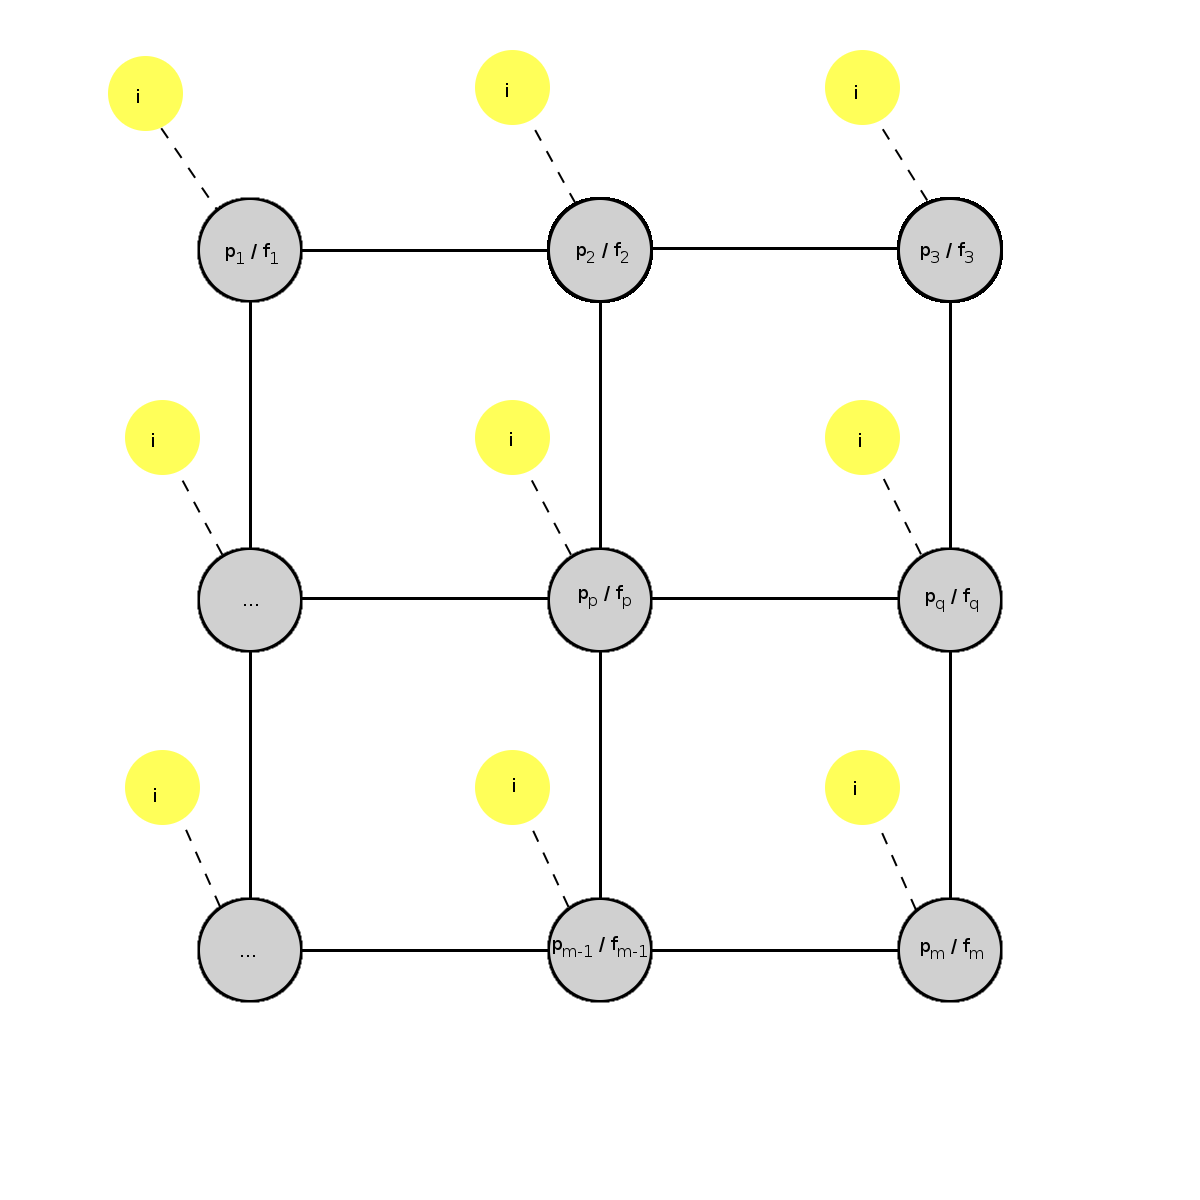
\includegraphics[width=1.15\textwidth]{/home/argo/seminar/mrf1.png}
\end{textblock}


\begin{textblock}{7}(7, 4.5)

\begin{itemize}
\item Condition for an MRF: Each random variable depends on other random variables only through its neighbors: \\

\vspace{0.25cm}

$p(f_p|f_{\mathcal{P} \setminus p}) = p(f_p|f_{\mathcal{N}_p}) $

\vspace{0.25cm}

\item here: neighborhood system are adjacent pixels

\end{itemize}

\end{textblock}

}

\frame{
\frametitle{Markov Random Fields (MRF) -- Prior/Binary term}



\begin{textblock}{7}(0., 4.)
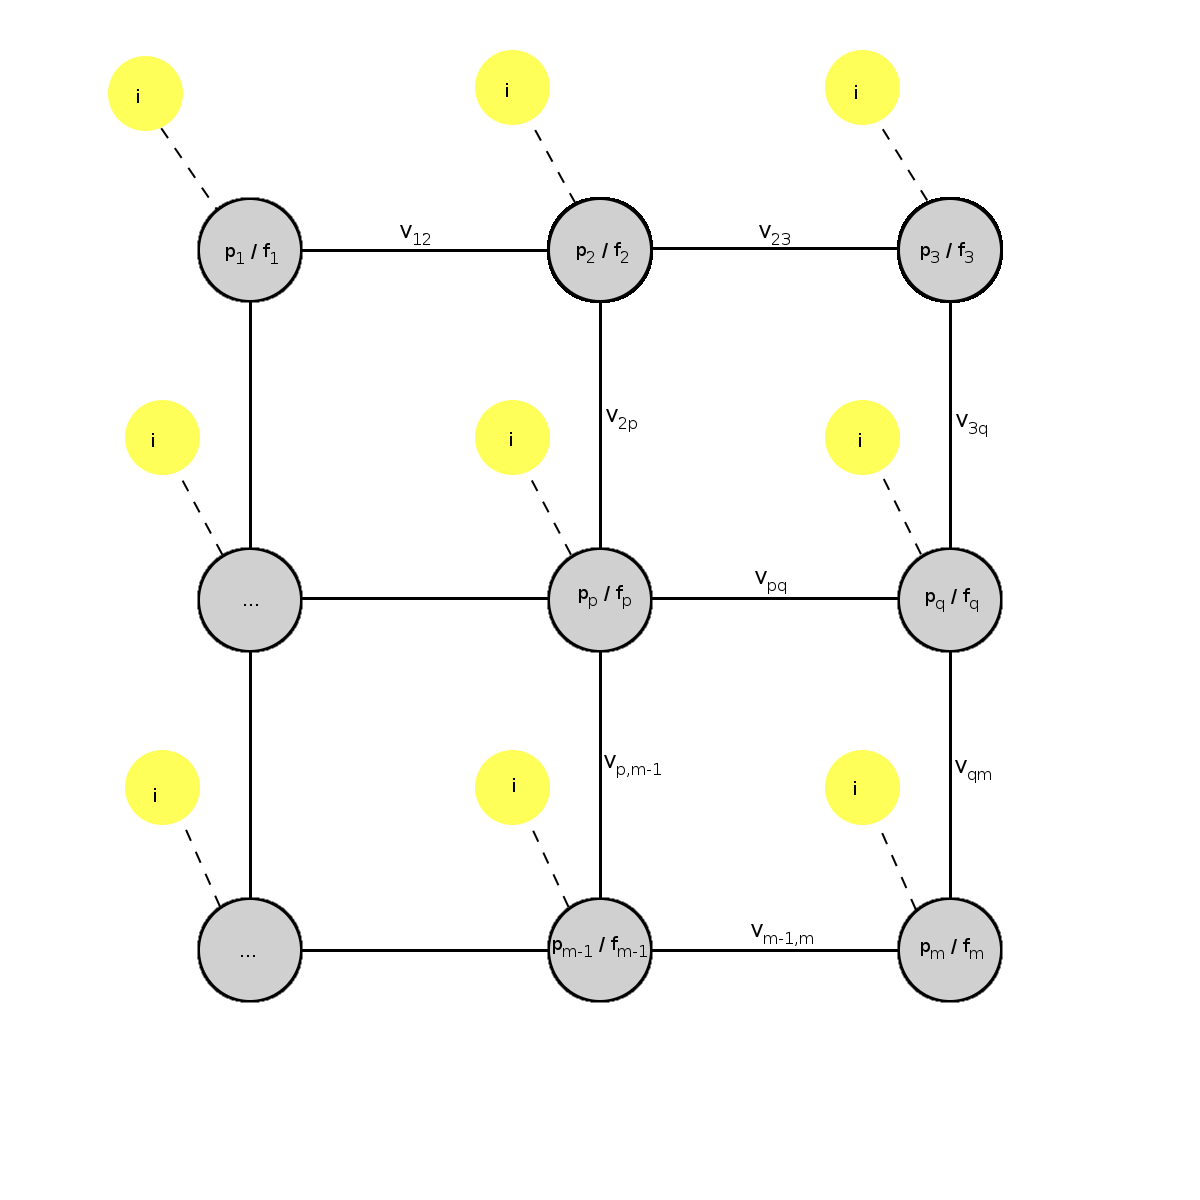
\includegraphics[width=1.15\textwidth]{/home/argo/seminar/mrf2.png}
\end{textblock}


\begin{textblock}{9}(7, 5.)

\begin{itemize}
	\item General for Markov Random Fields: \\
	Hammersley-Clifford theorem: $p(f) \propto \exp \{- \sum_C V_C(f) \}$ \\
	$C$: Clique in neighborhood system
	\vspace{0.25cm}
	\item Here: $p(f) \propto \exp\{ - \sum\limits_{p \in \mathcal{P}} \sum\limits_{q \in \mathcal{N}_p} V_{pq} (f_p, f_q) \}$
	\vspace{0.25cm}
	\item Used for smoothing to penalize different neighboring pixel labels.
\end{itemize}

\end{textblock}

}

\frame{
\frametitle{Markov Random Fields (MRF) -- Prior/Binary term}

\begin{textblock}{14}(1, 4.5)

Important example: Generalized Potts model \\

\begin{itemize}
	\item  $V_{pq}(f_p,f_q) = u_{pq}(1 - \delta(f_p - f_q))$
	\item Matrix notation: \\
	\vspace{-0.4cm}
	
	\renewcommand{\kbldelim}{(}% Left delimiter
	\renewcommand{\kbrdelim}{)}% Right delimiter
	\[
	  V_{pq} = \kbordermatrix{
	    & l_1 & l_2 & \dots & l_{k-1} & l_{k} \\
	    l_1   & 0 & u_{1,2} & \dots & u_{1,k-1} & u_{1,k} \\
	    l_2   & u_{2,1} & 0 & \ddots & \vdots & u_{2,k} \\
	    \vdots & \vdots & \ddots & \ddots & u_{...} & \vdots \\
	    l_{k-1}   & u_{k-1,1} & \dots & u_{...} & 0 & u_{k-1,k} \\
	    l_k   & u_{k,1} & u_{k,2} & \dots & u_{k,k-1} & 0 \\
	    }
	\]
	\vspace{0.1cm}
	\item Potts model is a metric, important for $\alpha$-expansion $\rightarrow$ later
\end{itemize}

\end{textblock}

}

\frame{
\frametitle{Markov Random Fields (MRF) -- Data/Unary term}

\begin{textblock}{7}(0., 4.)
\includegraphics[width=1.15\textwidth]{/home/argo/seminar/mrf3.png}
\end{textblock}

\begin{textblock}{9}(7, 5.)

\begin{itemize}
	\item Assume: i.i.d.\\
	\vspace{0.2cm}
	$p(O|f) = \prod\limits_{p \in \mathcal{P}} g(i_p, f_p)$
	
	\item Example:
	\begin{equation*}
	\hspace{-0.5cm}
	g(i_p,f_p) = \begin{cases}
		\exp(-|\bar{i}_1 - i_p|) & \text{for } f_p=l_1 \\
		\exp(-|\bar{i}_2 - i_p|) & \text{for } f_p=l_2 \\
	 	\quad \vdots \\
		\exp(-|\bar{i}_k - i_p|) & \text{for } f_p=l_k \\
		\end{cases}
	\end{equation*}
	
	\vspace{0.1cm}
	$\bar{i}_l$: average intensity label $l$
\end{itemize}

\end{textblock}

}

\frame{
\frametitle{Markov Random Fields (MRF) -- Energy formulation}

\begin{textblock}{14}(1, 4)

\begin{itemize}
\item Remember objective: $f^* = \arg \max\limits_{f} p(O|f) p(f) = \arg \min\limits_{f} E(f;i)$ \\

\item $p(O|f) = \prod\limits_{p \in \mathcal{P}} g(i, p, f_p)$ \\
\item $p(f) \propto \exp\{ - \sum\limits_{p \in \mathcal{P}} \sum\limits_{q \in \mathcal{N}_p} V_{pq} (f_p, f_q) \}$ \\

\item Insert these expressions and take negative logarithm:
\vspace{-0.2cm}
\begin{align*}
	E(f) & = - \ln(p(O|f) p(f)) \\
	& = \sum\limits_{p \in \mathcal{P}} \sum\limits_{q \in \mathcal{N}_p} V_{pq} (f_p, f_q) - \sum\limits_{p \in \mathcal{P}} \ln(g(i, p, f_p)) \\
	& \stackrel{e.g.}{=} \sum\limits_{p \in \mathcal{P}} \sum\limits_{q \in \mathcal{N}_p} V_{pq} (f_p, f_q) + \sum\limits_{p \in \mathcal{P}} \underbrace{|\bar{i}(f_p) - i_p|}_{D_p(f_p)}
\end{align*}




\end{itemize}

\end{textblock}

}


\frame{

\todo{Label-space reduction part ?!}

}


\subsection{Multiway Cut Problem}
\frame{
\frametitle{Multiway Cut Problem}

% will hier nur das Prinzip von nem Cut erklaeren und die wichtigsten Sachen
% Genaue weights kommen dann bei den 2 approx. Methoden

\begin{textblock}{8}(0.5, 4.5)
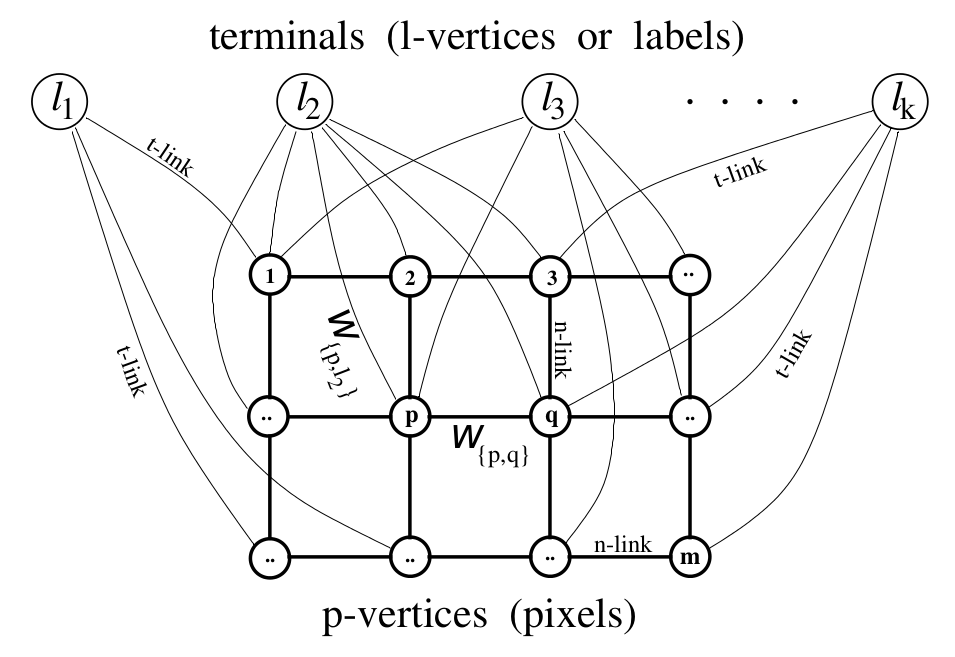
\includegraphics[width=1.2\textwidth]{/home/argo/seminar/data/general_multiway_cut_graph.png}
\end{textblock}


\begin{textblock}{6.}(9.5, 8.)

\begin{itemize}
	\item New graph \\ $\mathcal{G}_{mwc} = \langle\mathcal{N}_p \cup \mathcal{N}_t, \mathcal{E}_n \cup \mathcal{E}_t \rangle$
	\vspace{0.05cm} \\
	\item Weights are a function of prior- and data terms
\end{itemize}

\end{textblock}

}

\frame{
\frametitle{Multiway Cut Problem}

\begin{textblock}{12}(1., 4.5)
\textbf{Definition: \textit{multiway cut}}\\
A multiway cut is a subset $\mathcal{C} \subset \mathcal{E}$ of the graph's edges such that all terminals are no longer connected via edges in the induced graph $\mathcal{G}(\mathcal{C}) = \langle \mathcal{N}, \mathcal{E} - \mathcal{C}\rangle$.
 The cost of the cut $|\mathcal{C}|$ is the sum over all cutted edge's weights. 
 
 The minimum multiway cut problem is to find the multiway cut which minimizes $|\mathcal{C}|$. 
\end{textblock}

\begin{textblock}{12}(1., 11.)
\textbf{Definition: \textit{feasability multiway cut}}\\
A multiway cut is called feasible if each pixel node is left connected with exactly one terminal node in $\mathcal{G}(\mathcal{C})$. \\
\end{textblock}

}


\frame{
\frametitle{Multiway Cut Problem}

\todo{bild von jeweils nem multiway cut und einem feasible multiway cut um den unterschied zu verdeutlichen \\
$\rightarrow$ Tafel !!!}

}

\frame{
\frametitle{Multiway Cut Problem}

\begin{textblock}{12}(1., 4.5)
\textbf{Lemma:}\\
A minimum cost multiway cut $\mathcal{C}$ on $\mathcal{G}_{mwc}$ for terminals $\mathcal{L}$ must be feasible.

\end{textblock}

\begin{textblock}{12}(1., 8.)
\textbf{Theorem:}\\
If $\mathcal{C}$ is a minimum cost multiway cut on $\mathcal{G}_{mwc}$, then $f^\mathcal{C}$ minimizes $E(f)$.

\end{textblock}

}



\section{Approximative Algorithms}
\frame{
\frametitle{Approximative Algorithms}

\begin{textblock}{13}(1., 4.5)

\begin{itemize}
	\item Solving multiway cut problem exactly is NP-complete \\
	$\rightarrow$ exponential runtime in number of variables (pixels)
	\item Use approximative algorithms to achieve local minimum in reasonable time. \\
	\begin{itemize}
		\item Idea: Iteration with just two different labels in each step.
		\item $\rightarrow$ max-flow algorithm usable with near-linear complexity.
	\end{itemize}

\end{itemize}

\end{textblock}

}


\subsection{$\alpha$-$\beta$ swap}
\frame{
\frametitle{$\alpha$-$\beta$ swap}

\begin{textblock}{8}(1., 4.5)
\includegraphics[width=1.5\textwidth]{/home/argo/seminar/data/algorithm-alpha-beta-swap.png}
\end{textblock}


\begin{textblock}{13}(1., 13)

\textbf{Idea:} Loop over all pairs of labels and swap among them while ignoring all other labels 

\end{textblock}

}


\frame{
\frametitle{$\alpha$-$\beta$ swap -- min-cut subproblem}

\begin{textblock}{8}(0., 4.5)
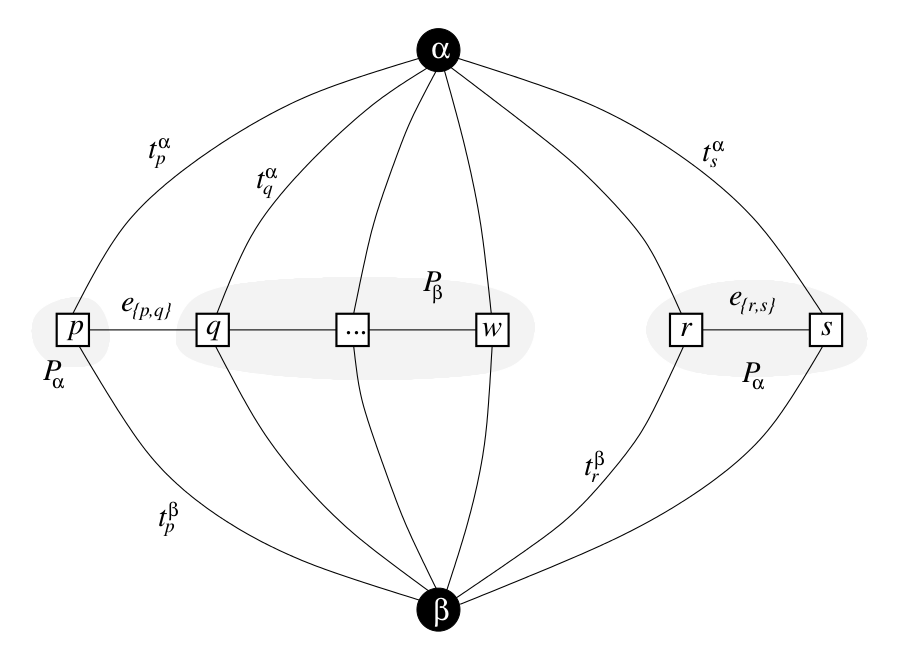
\includegraphics[width=0.8\textwidth]{/home/argo/seminar/data/alpha-beta-swap_Gab.png}
\centering \\
$\mathcal{G}_{\alpha \beta} = \langle \mathcal{N}_{\alpha \beta}, \mathcal{E}_{\alpha \beta} \rangle$
\end{textblock}

\begin{textblock}{7}(8., 4.5)

\begin{itemize}
	\item Graph just containts pixels with label $\alpha$ or $\beta$ and corresponding terminal nodes. 
	\vspace{0.2cm}
	\item Edge weights are as follows: \\
	\vspace{0.2cm}
	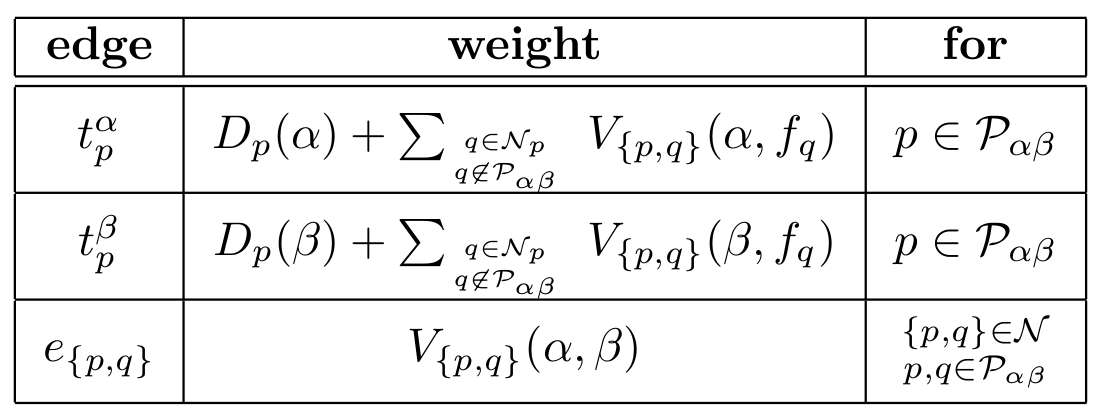
\includegraphics[width=0.9\textwidth]{/home/argo/seminar/data/alpha-beta-swap_weight-table.png}
\end{itemize}

\end{textblock}

}

\frame{
\frametitle{$\alpha$-$\beta$ swap -- min-cut subproblem}

\begin{textblock}{3}(1., 4.5)
		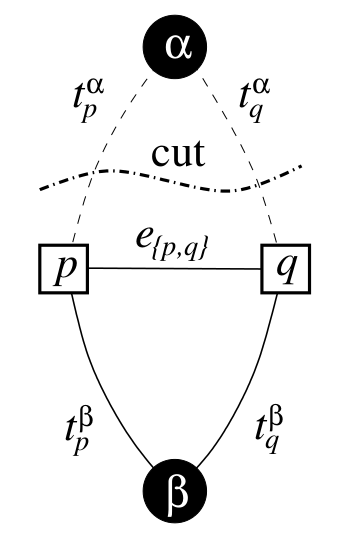
\includegraphics[width=1.\textwidth]{/home/argo/seminar/data/alpha-beta-swap_Gab_cut1.png}
		\centering \\
		$p, q \in \alpha$
\end{textblock}

\begin{textblock}{3}(6., 4.5)
		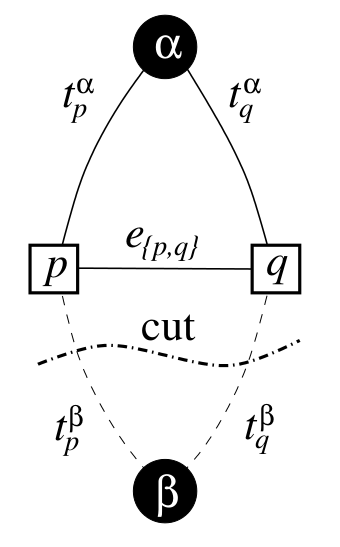
\includegraphics[width=1.\textwidth]{/home/argo/seminar/data/alpha-beta-swap_Gab_cut2.png}
		\centering \\
		$p, q \in \beta$
\end{textblock}

\begin{textblock}{3}(11., 4.5)
		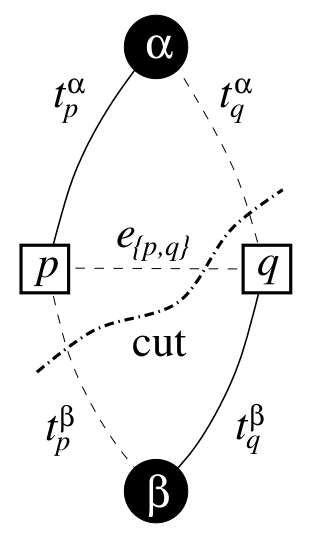
\includegraphics[width=0.945\textwidth]{/home/argo/seminar/data/alpha-beta-swap_Gab_cut3.png}
		\centering \\
		$p \in \beta$, $q \in \alpha$
\end{textblock}


\begin{textblock}{14}(1., 13.)
	\textbf{Careful:} Cutted terminal edge $t_p^\alpha$ means pixel $p$ gets label $\alpha$. \\
	Vice versa to general multiway cut problem!
\end{textblock}

}

\frame{
\frametitle{$\alpha$-$\beta$ swap -- min-cut subproblem}

\begin{textblock}{12}(1., 4.5)
\textbf{Theorem:}\\
There is a one to one correspondence between cuts $\mathcal{C}$ on $\mathcal{G}_{\alpha \beta}$ and labelings that are one $\alpha$-$\beta$ swap away from $f$. Moreover, the cost of a cut $\mathcal{C}$ on $\mathcal{G}_{\alpha \beta}$ is $|\mathcal{C}| = E(f^\mathcal{C})$ plus a constant. \\
\end{textblock}

\begin{textblock}{12}(1., 10.)
\textbf{Corollary:}\\
The optimal $\alpha$-$\beta$ swap from $f$ is $\hat{f} = f^\mathcal{C}$ where $\mathcal{C}$ is the minimum cut on $\mathcal{G}_{\alpha \beta}$. \\
\end{textblock}


}

\subsection{$\alpha$-expansion}
\frame{
\frametitle{$\alpha$-expansion}

\begin{textblock}{8}(1., 4.5)
\includegraphics[width=1.5\textwidth]{/home/argo/seminar/data/algorithm-alpha-expansion.png}
\end{textblock}


\begin{textblock}{13}(1., 12.5)

\textbf{Idea:} Loop over all labels (current one denoted as $\alpha$).  Considering all pixels, switch the pixel labels to $\alpha$ which minimizes $E(f)$.

\end{textblock}

}


\frame{
\frametitle{$\alpha$-expansion -- min-cut subproblem}

\begin{textblock}{8}(0., 3.8)
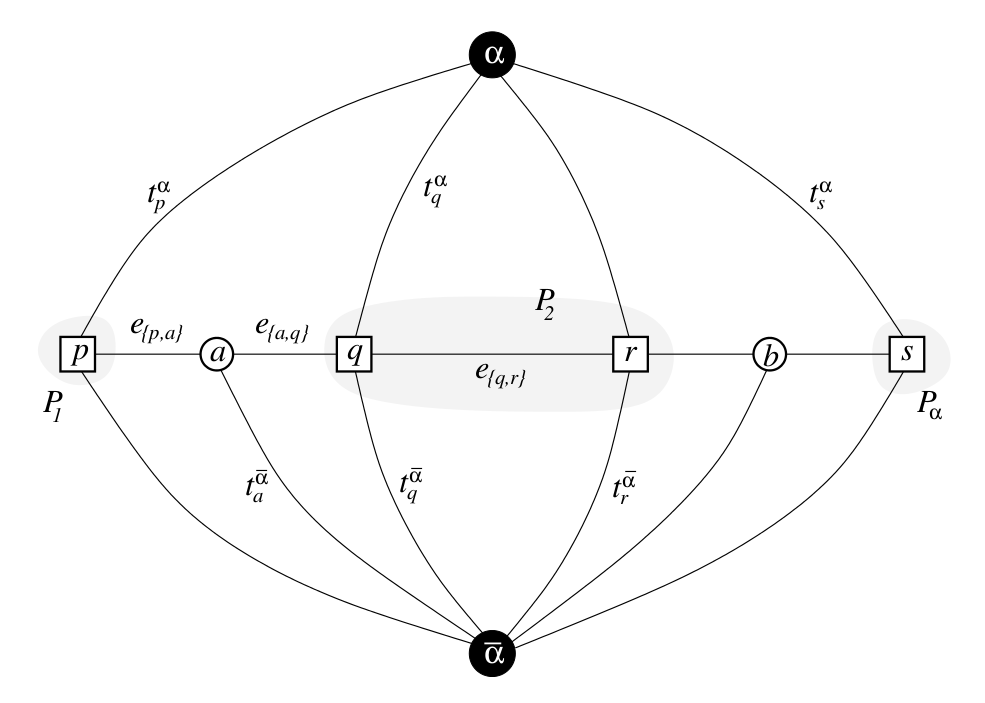
\includegraphics[width=0.8\textwidth]{/home/argo/seminar/data/alpha-expansion_G.png}
\centering \\
$\mathcal{G}_{\alpha}$ \\
\end{textblock}

\begin{textblock}{7}(8., 3.8)
\includegraphics[width=1.0\textwidth]{/home/argo/seminar/data/alpha-expansion_weight-table.png}
\end{textblock}


\begin{textblock}{14}(1., 11.3)
Graph contains
\begin{itemize}
	\item Terminal for both label $\alpha$ and one for all other labels $\bar{\alpha}$.
	\item Nodes for all pixels.
	\item Nodes between pixels with different labeling.
\end{itemize}
\end{textblock}

}


\frame{
\frametitle{$\alpha$-expansion -- min-cut subproblem}

\begin{textblock}{3}(1., 4.)
		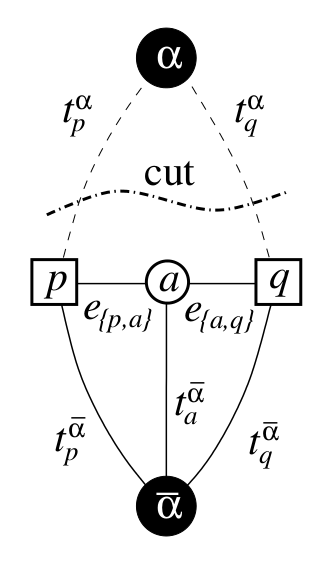
\includegraphics[width=1.\textwidth]{/home/argo/seminar/data/alpha-expansion_cut1.png}
		\centering \\
		$p, q \in \alpha$
\end{textblock}

\begin{textblock}{3}(6., 4.)
		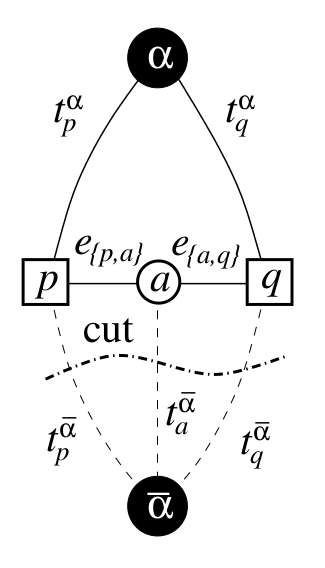
\includegraphics[width=1.\textwidth]{/home/argo/seminar/data/alpha-expansion_cut2.png}
		\centering \\
		$p, q$ keep previous label
\end{textblock}

\begin{textblock}{3}(11., 4.)
		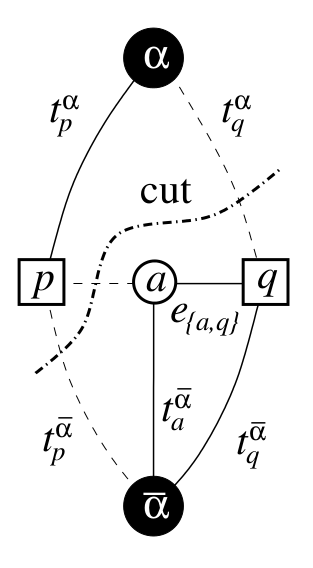
\includegraphics[width=0.945\textwidth]{/home/argo/seminar/data/alpha-expansion_cut3.png}
		\centering \\
		$q \in \alpha$ \\
		p keeps label
\end{textblock}


\begin{textblock}{14}(1., 13.5)
	\textbf{Careful:} Cutted terminal edge $t_p^\alpha$ means pixel $p$ gets label $\alpha$. \\
	Vice versa to general multiway cut problem!
\end{textblock}

}


\frame{
\frametitle{$\alpha$-expansion -- min-cut subproblem}

\begin{textblock}{6}(0.5, 4.5)
		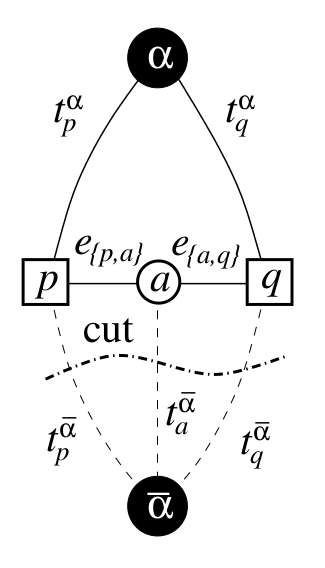
\includegraphics[width=0.45\textwidth]{/home/argo/seminar/data/alpha-expansion_cut2.png}
		\includegraphics[width=0.45\textwidth]{/home/argo/seminar/data/alpha-expansion_cut2_forbidden.png} \\
		\qquad \ $\surd$ \qquad \qquad \ \  X	
\end{textblock}


\begin{textblock}{9.5}(6., 4.)

\begin{itemize}
	\item Additional node $a$ required when both pixel keep their old label to include binary potential costs in cut cost $|t_a^{\bar{\alpha}}| = V(f_p, f_q)$.
	\vspace{0.15cm}

	\item One necessary condition: Potentials $V(f_p, f_q)$ must be a metric:
	\begin{itemize}
		\item $V(f_p, f_q) = V(f_q, f_p) \ge 0$
		\item $V(f_p, f_q) = 0 \Leftrightarrow f_p = f_q$
		\item $V(f_p, f_q) \le V(f_p, a) + V(a, f_q)$
	\end{itemize}
\end{itemize}

\end{textblock}


\begin{textblock}{14}(1., 12.5)
Second cut is forbidden because of metric propery

\vspace{-0.7cm}
\begin{align*}
	|t_a^{\bar{\alpha}}| \le |e_{(p,a)}| + |e_{(a,q)}| \qquad & \Leftrightarrow & 
	V(f_p, f_q) \le V(f_p, a) + V(a, f_q)
\end{align*}
\end{textblock}


}


\frame{
\frametitle{$\alpha$-expansion}

\begin{textblock}{12}(1., 4.5)
\textbf{Theorem:}\\
Let $\mathcal{G}_\alpha$ be construced as above given $f$ and $\alpha$. Then there is a one to one correspondence between elementary cuts on $\mathcal{G}_\alpha$ and labelings within one $\alpha$-expansion of $f$. Moreover, for any elementary cut $\mathcal{C}$ we have $|\mathcal{C}| = E(f^\mathcal{C})$.
\end{textblock}


\begin{textblock}{12}(1., 10.)
\textbf{Corollary:}\\
The optimal $\alpha$-expansion from $f$ is $\hat{f} = f^\mathcal{C}$ where $\mathcal{C}$ is the minimum cut on $\mathcal{G}_\alpha$. \\
\end{textblock}


}




\section{Application example}
\frame{
\frametitle{Application example}

\begin{textblock}{14}(1., 4.)

\begin{itemize}
	\item Software: OpenGM 2.0 from HCI, Heidelberg University \cite{opengm}
	\item 
\end{itemize}

\end{textblock}

}


\subsection{Flute segmentation}
\frame{
\frametitle{Flute segmentation}

\begin{textblock}{8}(1., 4.5)
		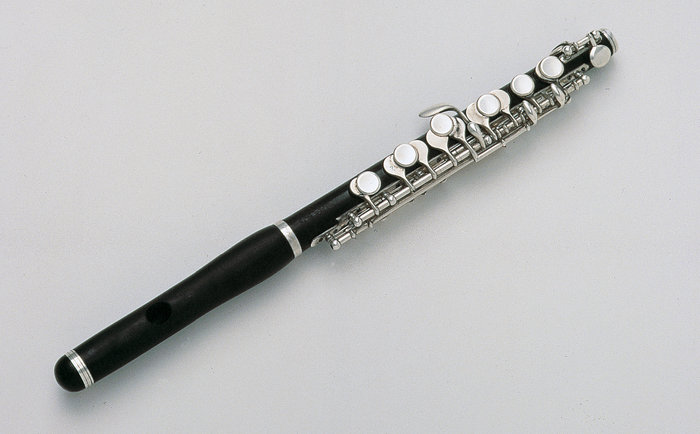
\includegraphics[width=1.\textwidth]{/home/argo/seminar/code/flute.jpg}
\end{textblock}


\begin{textblock}{6}(9., 4.5)

\begin{itemize}
	\item 3 different labels
	\vspace{0.2cm}
	\item Unary term: \\
	$D_p(f_p) = |\bar{i}(f_p) - i_p|$
	\item Binary term: \\
	$V_{pq} = (1 - \delta_{pq}) \cdot U$
	
\end{itemize}

\end{textblock}

\begin{textblock}{14}(1., 11.5)

\begin{itemize}
	\item $E(f) = \sum\limits_{p \in \mathcal{P}} \sum\limits_{q \in \mathcal{N}_p} V_{pq} (f_p, f_q) + \sum\limits_{p \in \mathcal{P}} {D_p(f_p)}$
\end{itemize}

\end{textblock}


}

\subsection{Depth Map estimation}
\frame{
\frametitle{Depth Map estimation}

\todo{Fragen ob als Beispiel auch ok...?}

}

\frame{
\frametitle{References}

\begin{textblock}{15}(0.5, 4.)


\begin{thebibliography}{9}

\bibitem{boykov98}
  Yuri Boykov, Olga Veksler and Ramin Zabih:
  Markov Random Fields with Efficient Approximations,
  1998,
  IEEE Computer Society Conference on Computer Vision and
  Pattern Recognition
  
\bibitem{boykov01}
  Yuri Boykov, Olga Veksler and Ramin Zabih:
  Fast Approximate Energy Minimization via Graph
  Cuts,
  IEEE Transactions on Pattern Analysis and Machine Intelligence archive Volume,
  23 Issue 11, November 2001 Page 1222-1239
  

\bibitem{opengm}
  OpenGM 2.0, Bjoern Andres, Thorsten Beier and Joerg H. Kappes, Heidelberg Collaboratory for Image Processing, University of Heidelberg
  
\bibitem{flute-img}
  \texttt{http://www.duden.de/\_media\_/ full/F/Floete-201100286673.jpg}

  

\end{thebibliography}

\end{textblock}
	
}
	
	
\end{document}